% 2007 年安徽卷理科第 14 题：抛物线 y=-x^2+1 与 x 轴正半轴交于 A，OA 的 n 等分点
%   P_1,P_2,...,P_{n-1} 处作垂线交抛物线于 Q_1,...,Q_{n-1}，得到 n-1 个直角三角形。
% 来源 PDF：gaokaomath-src/普通高考/2007/2007安徽理.pdf
% SHA-256：3f85f741d3b3790a308d698e4826ab196259643a8d40de12753c61cc6a9d2f0b
% 原页：2007安徽理.pdf 第 1 页（A3 三栏）第 2 栏，书页码 347，图在第 14 题题干下方。
% 重绘依据：横轴按 O 到 A 的实际区间作图（抛物线在 [0,1] 上单减），左端密排 P_1、P_2，
%   右端密排 P_{n-2}、P_{n-1} 与 A，中间以省略号断开；三角形 Q_1OP_1、Q_2P_1P_2、
%   Q_{n-1}P_{n-2}P_{n-1} 填浅灰，其余分点垂线只画到抛物线为止。
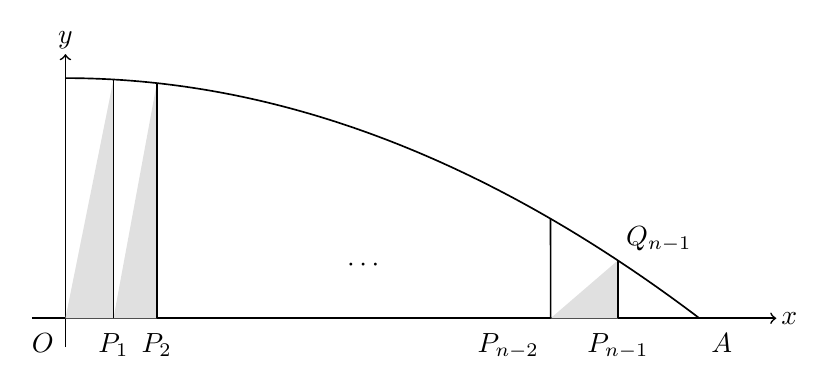
\begin{tikzpicture}[scale=1.22, semithick,
  every node/.style={inner sep=1.5pt}]
  \def\xA{6.6}
  \def\yy#1{2.5*(1-(#1/\xA)*(#1/\xA))}
  % 坐标轴
  \draw[->] (-0.35,0) -- (7.4,0) node[anchor=west] {$x$};
  \draw[->] (0,-0.3) -- (0,2.75) node[anchor=south] {$y$};
  % 抛物线
  \draw plot[domain=0:\xA, samples=120] (\x, {\yy{\x}});
  % 左端分点
  \coordinate (O)  at (0,0);
  \coordinate (P1) at (0.5,0);
  \coordinate (P2) at (0.95,0);
  \coordinate (Q1) at (0.5,{2.5*(1-(0.5/6.2)^2)});
  \coordinate (Q2) at (0.95,{2.5*(1-(0.95/6.2)^2)});
  % 右端分点
  \coordinate (Pn2) at (5.05,0);
  \coordinate (Pn1) at (5.75,0);
  \coordinate (A)   at (6.6,0);
  \coordinate (Qn1) at (5.75,{2.5*(1-(5.75/6.6)^2)});
  % 直角三角形填色
  \fill[black!12] (O) -- (P1) -- (Q1) -- cycle;
  \fill[black!12] (P1) -- (P2) -- (Q2) -- cycle;
  \fill[black!12] (Qn1) -- (Pn2) -- (Pn1) -- cycle;
  % 分点垂线
  \draw (P1) -- (Q1);
  \draw (P2) -- (Q2);
  \draw (Pn2) -- (5.05,{2.5*(1-(5.05/6.6)^2)});
  \draw (Pn1) -- (Qn1);
  % 省略号
  \node at (3.1,0.55) {$\cdots$};
  % 标注
  \node[anchor=north east] at ([xshift=-2pt,yshift=-3pt]O)  {$O$};
  \node[anchor=north] at ([yshift=-3pt]P1) {$P_1$};
  \node[anchor=north] at ([yshift=-3pt]P2) {$P_2$};
  \node[anchor=north east] at ([xshift=-2pt,yshift=-3pt]Pn2) {$P_{n-2}$};
  \node[anchor=north] at ([yshift=-3pt]Pn1) {$P_{n-1}$};
  \node[anchor=north west] at ([xshift=2pt,yshift=-3pt]A) {$A$};
  \node[anchor=south west] at ([xshift=1pt,yshift=1pt]Qn1) {$Q_{n-1}$};
\end{tikzpicture}
